%%%%%%%%%%%%%%%%%%%%%%%%%%%%%%%%%%%%%%%%%%%%%%%%%%%%%%%%%%%%%%%%%%
%%%%%%%% ICML 2015 EXAMPLE LATEX SUBMISSION FILE %%%%%%%%%%%%%%%%%
%%%%%%%%%%%%%%%%%%%%%%%%%%%%%%%%%%%%%%%%%%%%%%%%%%%%%%%%%%%%%%%%%%

% Use the following line _only_ if you're still using LaTeX 2.09.
%\documentstyle[icml2015,epsf,natbib]{article}
% If you rely on Latex2e packages, like most moden people use this:
\documentclass{article}

% use Times
\usepackage{times}
% For figures
\usepackage{graphicx} % more modern
%\usepackage{epsfig} % less modern
\usepackage{subfigure} 
\usepackage{amsmath,amsfonts,amssymb,bbm}

% For citations
\usepackage{natbib}

% For algorithms
\usepackage{algorithm}
\usepackage{algorithmic}

% As of 2011, we use the hyperref package to produce hyperlinks in the
% resulting PDF.  If this breaks your system, please commend out the
% following usepackage line and replace \usepackage{icml2015} with
% \usepackage[nohyperref]{icml2015} above.
\usepackage{hyperref}

% Packages hyperref and algorithmic misbehave sometimes.  We can fix
% this with the following command.
\newcommand{\theHalgorithm}{\arabic{algorithm}}
\DeclareMathOperator{\Tr}{Tr}
\newcommand{\R}{\mathbbm{R}}
\newcommand{\mba}{\mathbf{a}}
\newcommand{\mbb}{\mathbf{b}}
\newcommand{\mbx}{\mathbf{x}}
\newcommand{\mbxt}{\tilde{\mathbf{x}}}
\newcommand{\Sigmat}{\tilde{\Sigma}}
\newcommand{\mbz}{\mathbf{z}}
\newcommand{\mbw}{\mathbf{w}}
\newcommand{\mcN}{\mathcal{N}}
\newcommand{\mcP}{\mathcal{P}}
\newcommand{\eps}{\epsilon}
\newcommand{\trans}{\intercal}
\newcommand{\Ut}{\tilde{U}}
\DeclareMathOperator*{\argmax}{arg\,max}
\newcommand{\angstrom}{\textup{\AA}}
\newcommand{\red}[1]{\textcolor{red}{[TODO: #1]}}


% Employ the following version of the ``usepackage'' statement for
% submitting the draft version of the paper for review.  This will set
% the note in the first column to ``Under review.  Do not distribute.''
%\usepackage{icml2015} 

% Employ this version of the ``usepackage'' statement after the paper has
% been accepted, when creating the final version.  This will set the
% note in the first column to ``Proceedings of the...''
\usepackage[accepted]{icml2015}


% The \icmltitle you define below is probably too long as a header.
% Therefore, a short form for the running title is supplied here:
\icmltitlerunning{Model of Quasar Spectroscopy}

\begin{document} 

\twocolumn[
\icmltitle{A Stochastic Process Model of Quasar Spectroscopy} %# \\
%Inference of Red Shift from Quasar Photometry }

% It is OKAY to include author information, even for blind
% submissions: the style file will automatically remove it for you
% unless you've provided the [accepted] option to the icml2015
% package.
\icmlauthor{Andrew Miller}{acm@seas.harvard.edu}
\icmlauthor{Albert Wu}{awu@college.harvard.edu}
\icmladdress{Harvard University,
             33 Oxford St, Cambridge, MA USA}
\icmlauthor{David Schlegel}{djschlegel@lbl.gov}
\icmladdress{Lawrence Berkeley National Laboratory, 
             1 Cyclotron Road, Berkeley, CA, 94720 USA}
\icmlauthor{Ryan Adams}{rpa@seas.harvard.edu}
\icmladdress{Harvard University,
             33 Oxford St, Cambridge, MA, 02138 USA}

             
% You may provide any keywords that you 
% find helpful for describing your paper; these are used to populate 
% the "keywords" metadata in the PDF but will not be shown in the document
\icmlkeywords{boring formatting information, machine learning, ICML}

\vskip 0.3in
]

\begin{abstract} 
We describe a method for combining information from two disparate sources of astronomical data, spectroscopy and photometry, which carry information about sources of light (e.g.~stars, galaxies, quasars) at extremely different resolutions. 
Our model treats the spectral energy distribution (SED) of the radiation of a source as a latent variable, hierarchically generating both photometric and spectroscopic observations.  
Furthermore, we view the problem of SED inference as a density estimation problem, placing a flexible nonparametric prior over the SED of a light source that admits a physically interpretable decomposition and allows us to tractably perform fully Bayesian inference using MCMC.  
We exhibit the utility of our model by using it to predict the distribution of the red-shift of quasars from five-band (low resolution) photometric data, the so called ``photo-z'' problem. 
Our method shows that tools from machine learning and Bayesian statistics can allow us to jointly model multiple resolutions of information to make accurate predictions with well-characterized uncertainties.  
%Our method leverages a small number of existing examples of high resolution quasar spectra with known red-shift to build a structured prior distribution over unknown spectra.  
%We describe a fully generative model that combines information from a large dataset of high resolution spectroscopic measurements with a small number of broadband photometric observations, and we use it to measure the red-shift of quasars from photometry, the ``photo-z'' problem.  
\end{abstract} 

\section{Introduction}
Enormous amounts of astronomical data are collected by a range of instruments at multiple resolutions, providing information about billions of sources of light in the observable universe. \red{cite sloan digital sky survey, other astronomical surveys}.  
Among this collection of data are measurements of the spectral energy distribution (SED) of a source.  
The SED describes the distribution of energy radiated by a source over the spectrum of wavelengths or energy levels.  
For intuition, the SED of a star at around $5,800\, K$ (like our sun) radiates most of it's energy in the $4,000 \angstrom$ to $7,000\angstrom$ range, which corresponds roughly to the range of visible light.  
However, stars tend to have simple distributions (well-modeled by Planck's law), whereas other objects, such as galaxies and quasars, can have much more complicated SEDs.  
The SED of a source is an object of interest because it carries information about the physical properties of the particular object, which can include type of source, effective temperature, distance to earth, and red-shift. 

Measurements of SEDs, however, are produced by instruments at widely varying resolutions.  
Spectroscopic measurements can can resolve noisy measurements of a source's SED in finer detail than broadband photometric measurements.  For example, the Baryonic Oscillation Spectroscopic Survey \cite{dawson2013baryon} measures SED samples at over four thousand wavelengths between 3,500 and 10,500 $\angstrom$.  
In contrast, the photometry from the Sloan Digital Sky Survey (SDSS) \red{cite sloan}, gathers broadband photometric measurements in the $u,g,r,i,$ and $z$ bands.  These measurements are the weighted average response over a large swath of the wavelength spectrum, often expressed as a vector of band-specific fluxes, roughly corresponding to the number of photons measured over the area and duration of an exposure.  
The two methods of spectral information collection are compared in Figure~\ref{fig:filters}. 

Despite carrying less information, broadband photometric measurements are more widely available and exist for a larger number of sources than spectroscopic measurements. 
This work develops a method for extracting information from observations of light sources by \emph{jointly} modeling spectroscopic and photometric data.  
In particular, we we focus on measuring the red-shift of quasars for which we only have photometric observations.  
Quasars, or quasi-stellar radio sources, are extremely distant and energetic sources of electromagnetic radiation that can exhibit high red-shift \red{cite something here}.  
Estimates and accurate characterization of uncertainty of red-shift measurements from photometry have the potential to guide the study of certain quasars with higher resolution instruments.  
Furthermore, accurate models can aid the automation of identifying and classifying faintly observed quasars in large photometric surveys.  
%Identifying and measuring the red-shift of a quasars from photometric data is a necessary task due to the widespread availability of large photometric surveys.  

%Study of distant quasars allow astronomers to observe the universe as it was many billions of years ago \red{need lots of references.}. 
In this paper, we describe a probabilistic model that jointly describes both high resolution spectroscopic data and low resolution photometric observations of quasars in terms of their latent SEDs, luminosity, and red-shift.  We model a quasar's spectral energy as a latent variable, and describe a fully Bayesian inference procedure to compute the marginal probability distribution of a quasar's red-shift given observed photometric fluxes and their uncertainties.  The following section provides relevant application and statistical background, as well as related work on the ``photo-z'' problem.  Section~\ref{sec:model} describes our probabilistic model of SEDs and broadband photometric measurements.  Section~\ref{sec:inference} outlines our MCMC-based inference method for efficiently computing statistics of the posterior distribution. Section~\ref{sec:experiments} presents red-shift and SED predictions from photometric measurements, among other model summaries.    

\section{Background}
\label{sec:background}
The SED of an object describes the distribution of energy it radiates as a function of wavelength.  
For example, most stars are well modeled as a blackbody, so their spectral radiance closely follows Planck's law, which describes a parametric form for the spectral energy distribution.  Resolvable stars, however, tend to be close enough that they are never observed at a non-zero redshift. 
Quasars, on the other hand, have a complicated spectral energy distribution characterized by some salient features (\red{mention Ly-$\alpha$ and Lyman forest?}).  
Furthermore, quasars can be much more luminous and at a much higher red-shift.  
The effect of red-shift is the stretching of the input space of wavelengths, $\lambda\in \Lambda$, of an object's \emph{rest-frame} SED toward longer wavelength values, skewing its mass toward longer (redder) wavelengths. 
Denoting the rest-frame SED of a quasar $n$ as a function, $f_n^{(rest)} : \Lambda \rightarrow \R_+$, the affect of red-shift on our observations is summarized by the relationship 
\begin{align}
  f_n^{(obs)}(\lambda) &\propto f_n^{(rest)}(\lambda \cdot (1 + z_n)) \, .
\end{align}
Observed quasar spectra and their ``de-red-shifted'' rest frame spectra are depicted in Figure~\ref{fig:frames}

%% example of obs vs rest frame data
\begin{figure*}[ht]
\vskip 0.2in
\begin{center}
\centerline{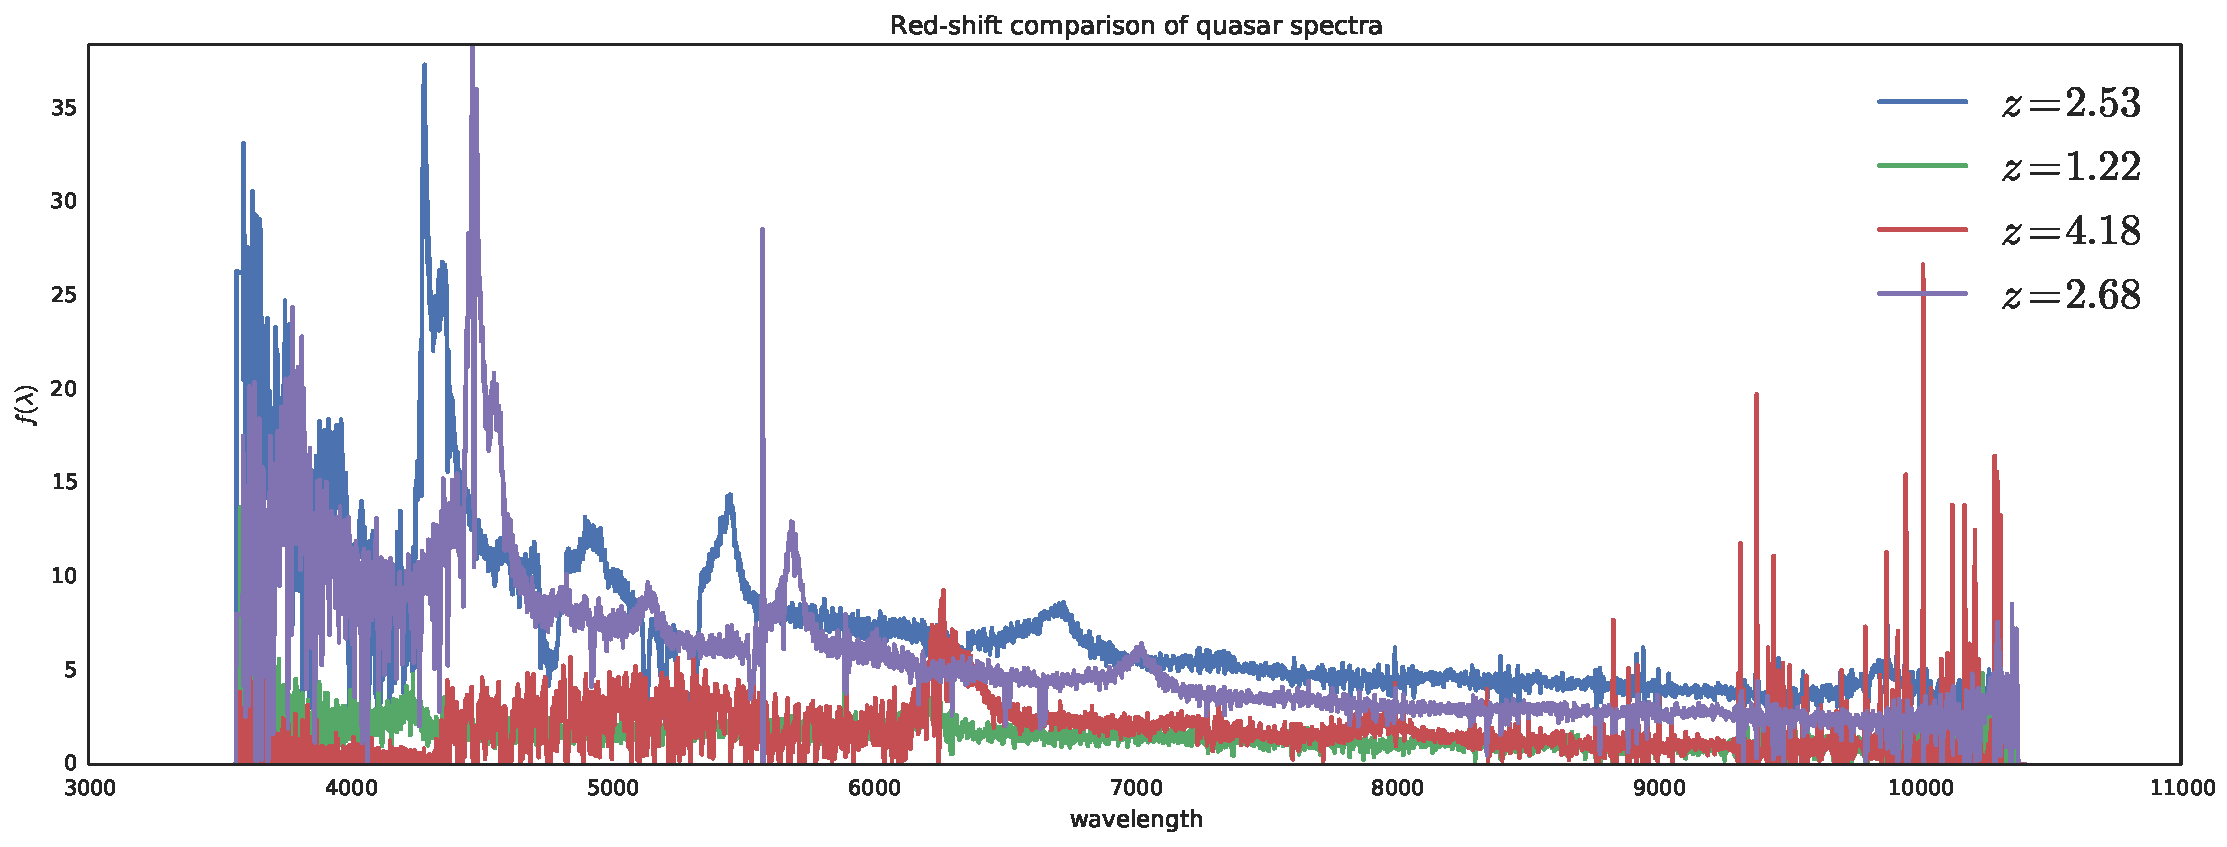
\includegraphics[width=2\columnwidth]{../figs/quasar_redshift_obs_frame}}
\centerline{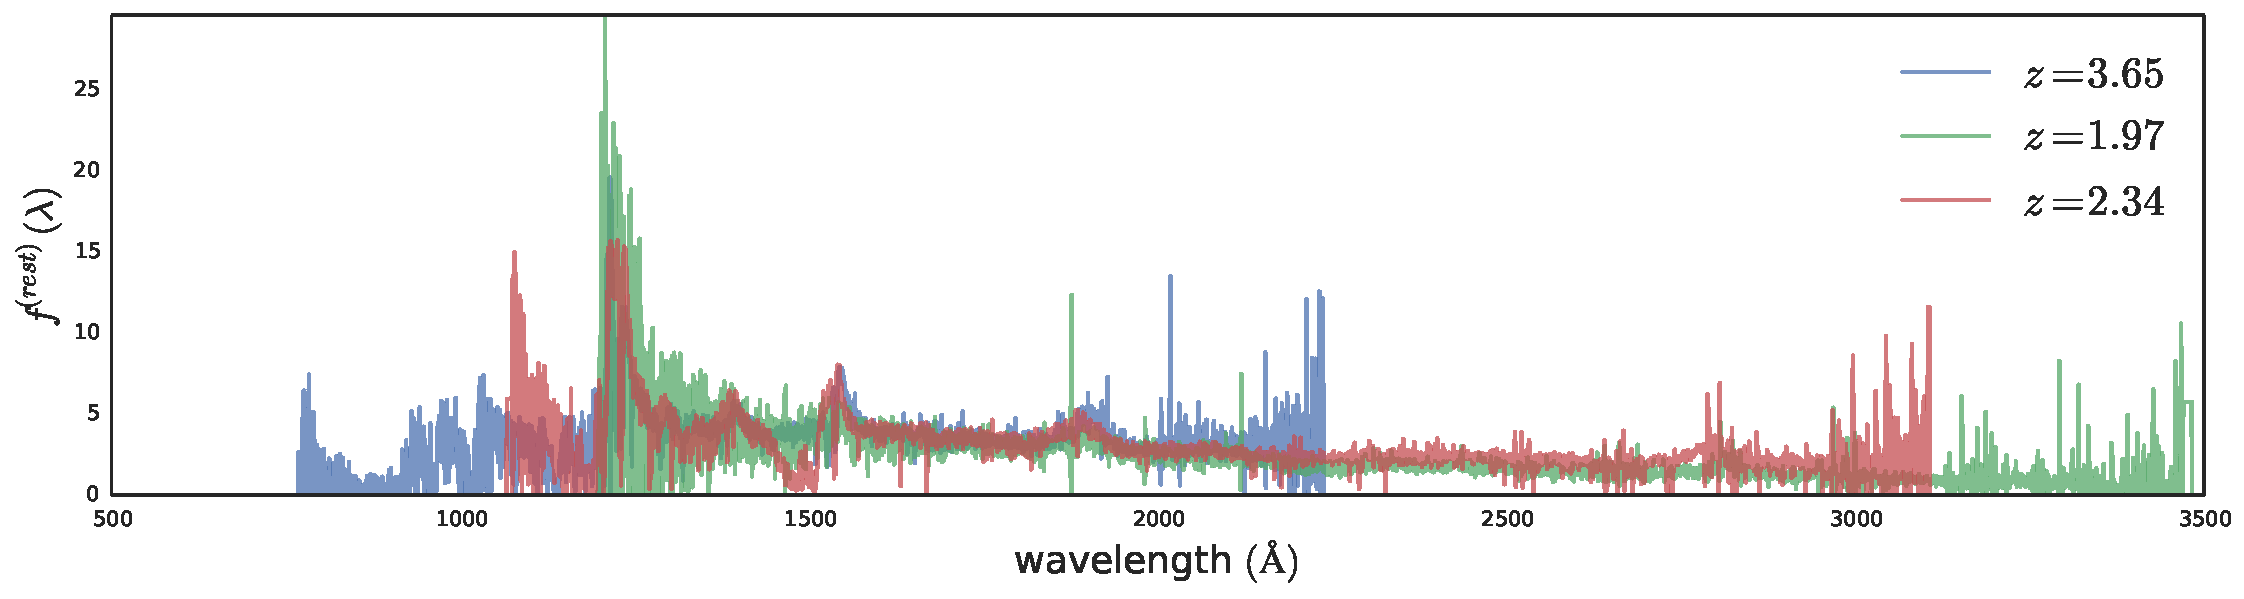
\includegraphics[width=2\columnwidth]{../figs/quasar_redshift_rest_frame}}
\caption{High fidelity spectroscopy of multiple quasars at different red-shifts, $z$.  The top graphic depicts the spectrograph in the observation frame, which can be intuitively thought of as ``stretched'' by a factor $(1+z)$.  The lower figure depicts the ``de-redshifted'' version of the same quasar spectra.  This effectively squashes observations, and reconstructs the quasar spectra as it would be seen in the quasar's rest frame.  The salient feature of this operation is the alignment of the emission and absorption lines (albeit at different scales).  This alignment will provide the information about $z$ that we can infer from SDSS photometric projections of the very same spectra.}
\label{fig:frames}
\end{center}
\vskip -0.2in
\end{figure*} 

\subsection{Related work}
The problem of estimating the red-shift of a source (galaxy or quasar) is known as photometric redshift estimation, or
``photo-$z$''.  There have been many statistical and machine learning methods developed to tackle this problem. These roughly break down into template-based and regression-based methods. Template-based methods use prior knowledge from spectral energy distributions
and match these with actual astronomical objects, while regression-based methods use fitting methods, such as neural networks and
simple regression, on the physical properties to predict red shift. \cite{walcher2011fitting}.  Regression-based (or empirical) methods for photo-$z$ fit a functional relationship between a set of photometric features and red-shift value.  

Probabilistic models for inferring red-shift from photometry have also had some success.  \cite{benitez2000bayesian} presents a thorough summary of Bayesian methods for photometric red-shift estimation from spectral templates.  

\cite{budavari2001photometric} and \cite{richards2001photometric} go into specific detail for SED model based photometric redshifts for quasars.  They compare a bunch of methods. Particularly, they describe an algorithm for reconstruction a quasar spectrum template from photometric observations and spectroscopic redshifts.  It seems sorta like a dynamic K-means/EM algorithm (they add spectral types as needed), and does a decent job reconstructing bumps where the emission lines are.  

\cite{brescia2013photometric} use a multi-layer perceptron with a combination of SDSS, UKIDSS, and WISE photometric fluxes datasets, to compute a regression function for red-shift. Though predictions are accurate, we do not have an idea of the distribution over redshifts, i.e., uncertainty in our predictions.

Other models blur the line between regression-based and generative models.  \cite{bovy2012photometric} develops a method termed $XDQSOz$ to use a large dataset of astronomical objects to simultaneously infer redshift and classify quasars. They do this by inferring a joint distribution over object type, fluxes, and redshift. In particular, they factor this joint distribution
into one part that describes the distribution over star brightness, which involves binning based on a single-channel flux, and
one part that describes the distribution of relative fluxes (as compared to this channel) and the redshift. The latter distribution
is represented by a mixture of up to 60 Gaussians. However, we see that, due to the
binning, this approach is not fully probabilistic or Bayesian.


\cite{budavari2009unified} unifies template-based and regression-based
approaches into a single probabilistic framework, distinguishing methods based on the assumptions they impose on probability distributions over photometric fluxes. Instead of treating the spectral distribution and physical properties as disparate, the authors represent physical properties as a random variable whose conditional distributions over observations such as spectra can be computed.

\red{Others to mention: }
\cite{suzuki2006quasar} does unsupervised learning on the UV spectra of quasars using principal components analysis (PCA). Through this analysis, the authors found that 96\% of the total variance was accounted for by the first 3 spectral components. As a result, they created a classification scheme based on the first two component's coefficients that separates quasars into five different classes. This classification scheme allows researchers to understand quasars better from a qualitative perspective.

\red{This doesn't seem that relevant. What do you think, Andy?}


%----------------------------------------------------------------------------------
%----------------------------------------------------------------------------------
%----------------------------------------------------------------------------------
\section{Model}
\label{sec:model}
This section describes the details of our probabilistic model for spectroscopic and photometric observations.  

\subsection{Stochastic Process Model of Spectra}
The SED of a quasar is a nonnegative valued function $f : \Lambda \rightarrow \R^+$, where $\Lambda$ denotes the range of wavelengths and $\R^+$ are nonnegative real-valued numbers.  However, the types of spectra we observe from quasars is highly structured, and we use an additive decomposition of a small number of positive bases (or templates) to capture this structure.   We model a quasar's SED \emph{in rest-frame} as a positive linear combination of a set of positive basis functions.  Interpreting the spectra as a scaled probability distribution, we model it as a random measure.  We place a log-Gaussian process prior on each of these basis functions, and a prior over positive weight values for each quasar.  
\red{Todo: include brief GP background}

The generative procedure for quasar spectra is first generate a shared positive basis
\begin{align}
  \beta_k(\cdot) &\sim \mathcal{GP}(0, K_\theta) \, , k=1, \dots, K\\
  B_k(\cdot) &= \frac{\exp(\beta_k(\cdot))}{\int_\Lambda \exp(\beta_k(d \lambda))}   
\end{align}
and for each quasar, $n$
\begin{align}
  \mathbf{w}_n &\sim p(\mathbf{w}) \, , \text{ s.t. } \sum_{w_k} = 1  \\
  m_n  &\sim p(m) \, \text{ s.t. } m_n > 0 \\
  f^{(rest)}_n(\cdot) &= \sum_{k} w_k B_k(\cdot) &&\text{ (SED) }\\
  \tilde f^{(rest)}_n(\cdot) &= m_n \sum_{k} w_k B_k(\cdot) \\
  z_n &\sim p(z) &&\text{(red-shift)}
\end{align}
where $p(\mathbf{w})$ is a prior over weights that sum to one, and $p(z)$ is a prior over red-shifts. 

Each positive basis function, $B_k$ is normalized to integrate to one, and each quasar's weight vector $\mathbf{w}_n$ also sums to one.  This allows us to interpret the $f^{(rest)}_n(\cdot)$ function as a density, scaled by $m_n$. 
\red{Todo: Warp input for varying lengthscale}.  

For each quasar $n$, we observe noisy samples of the red-shifted and scaled spectral energy distribution at a grid of wavelengths $\lambda \in \{\lambda_1, \dots, \lambda_P \}$.  Our \emph{observation frame} samples are modeled
\begin{align}
  x_{n, \lambda} 
    &\sim \mathcal{N}\left( \frac{1}{(1 + z_n)} \tilde f_n^{(rest)}( \lambda \cdot (1 + z_n) ), \sigma_{n,\lambda}^2 \right)
    \label{eq:spec} 
\end{align}
where $\sigma_{n, \lambda}^2$ is known instrument variance. The BOSS spectra (and our rest-frame bassi) are stored in units ergs/cm$^2$/s/$\angstrom$. 

\subsection{Photometric Observations}
Photometric observations summarize the number of photon observations over a large swatch of the wavelength spectrum.  Roughly, a photometric flux measures the number of photons hitting the instrument's lens, filtered by a band-specific sensitivity curve, over the duration of an exposure. 
We will express measurements of flux in nanomaggies \red{reference}, a linear unit of flux, in our method and experiments.  
The photometric data are measured in the SDSS $ugriz$ bands, giving us a vector, $\mathbf{y}_n$, of five flux values and their variances, $\tau_{n, b}$ for $b \in ugriz$, which are computed from images. \red{PSFFLUX - those are straight from pixels???}.  
Each band measures photon observations at each wavelength in proportion to a known filter sensitivity, $S_{band}(\lambda)$. 
The filter sensitivities for the SDSS $ugriz$ bands are depicted in Figure~\ref{fig:filters}, with an example (observation frame) quasar spectrum overlaid.   The actual measured fluxes can be computed by integrating the full object's spectrum, $m_n \cdot f_n(\lambda)$ against the filters.  For a band $b \in \{u, g, r, i, z \}$
\begin{align}
  \mu_b &= \int f^{(obs)}_n(\lambda) S_b(\lambda) C(\lambda) d \lambda  \\
        &\equiv I_b(f_n^{(rest)}, z_n)
\end{align}
where $C(\lambda)$ is a conversion factor to go from the units of $f_n(\lambda)$ to nanomaggies.  This projection onto SDSS bands results in five fluxes, which are modeled as independent Gaussian random variables with known variance (derived from a pixel to flux inference procedure)
\begin{align}
  y_{n,b} &\sim \mathcal{N}( I_b(f_n^{(rest)}, z_n), \tau_{n,b} )
  \label{eq:phot}
\end{align}
Given a low dimensional summary of $f_n^{(rest)}$, we can rewrite $I$ as a function of those parameters. 

\subsection{Joint model}
Given a sample of $M$ noisy full spectra and their sample locations, $\{\mathbf{x}_m, \lambda^{(obs)}_m \}_{m=1}^M$, and a set of $N$ photometric fluxes, $\{\mathbf{y}_n\}_{n=1}^N$, our full likelihood in terms of $\{ \mathbf{w}_m \}_{m=1}^M, B_1, \dots, B_K, \{ w_n \}_{n=1}^N$, and $\{z_m\}, \{z_n\}$ is 
\begin{align*}
  L( \{ \mathbf{w}_m, z_m \}, &\{ B_k \}, \{ \mathbf{w}_n, z_n \} )  \\
    = & \prod_{m=1}^M p( \mathbf{x}_m | \mathbf{w}_m, z_m, \{ B_k \})  \\
      & \times \prod_{n=1}^N p( \mathbf{y}_n | \mathbf{w}_m, z_m, \{ B_k \})
\end{align*}
where the probability distribution of the first term in the product is given by \ref{eq:spec}, and the distribution for the second term in the product is given by \ref{eq:phot}.  

We express the joint prior distribution over the quasar weights $\mathbf{w}_n$ and $\mathbf{w}_m$ and basis 
\begin{align}
  p( \{ \mathbf{w}_m, z_m \}, &\{ B_k \}, \{ \mathbf{w}_n, z_n \} )  \\
    = & p(\{ B_k \}) p( \{ \mathbf{w}_m, z_m \} )  \\
      & p( \{ \mathbf{w}_n, z_n \} | \{ \mathbf{w}_m, z_m \} ) 
\end{align}
where we condition the photometric weights on the spectroscopically fit weights.  

\begin{figure*}[ht]
\vskip 0.2in
\begin{center}
\centerline{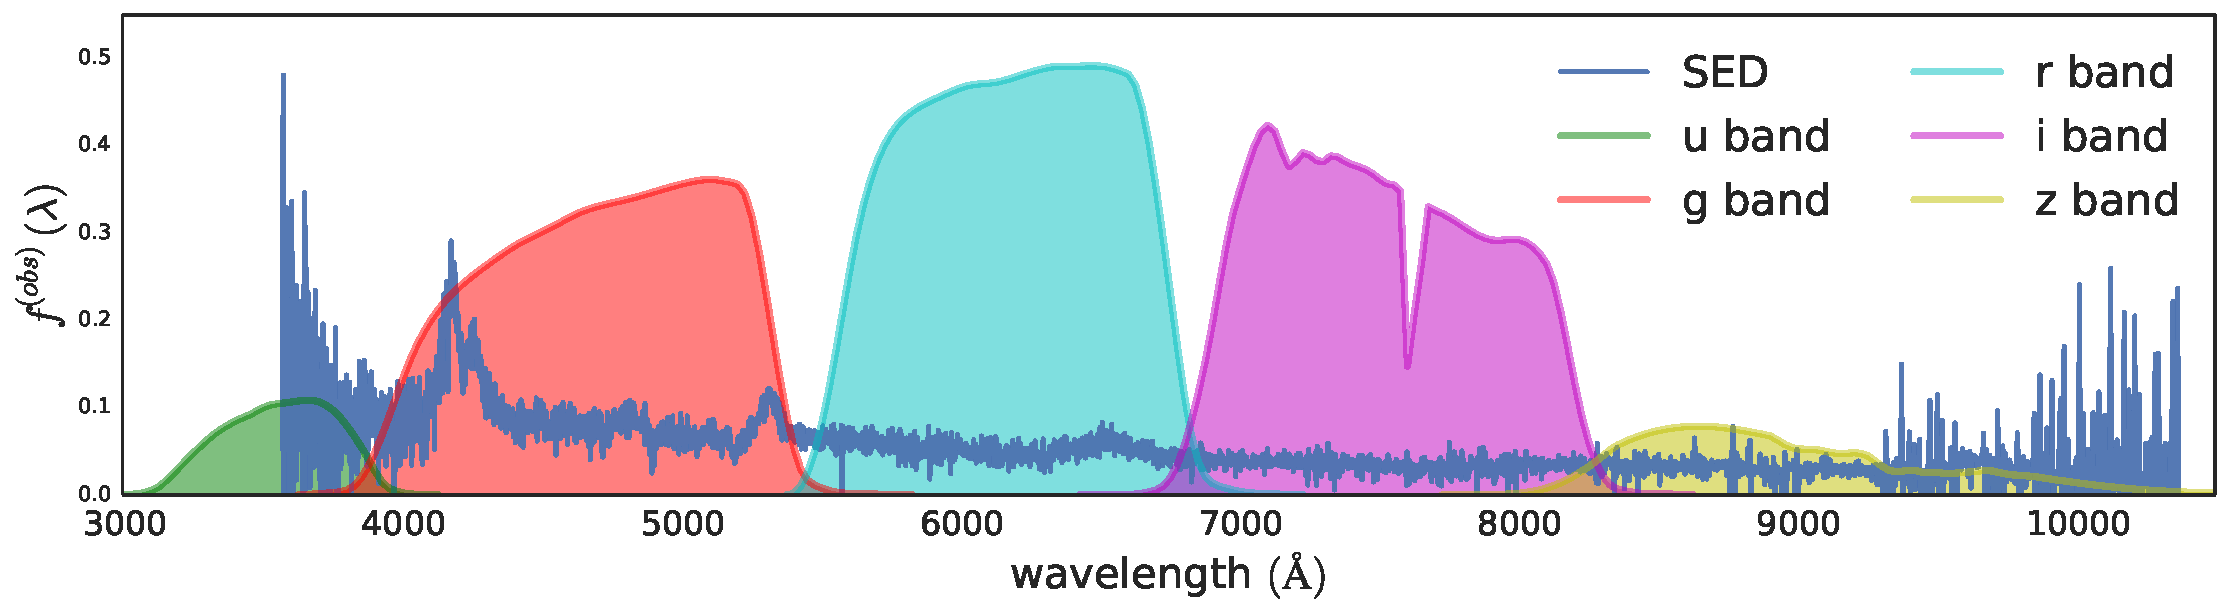
\includegraphics[width=2\columnwidth]{../figs/quasar_spectrum_sdss_filters}}
\caption{Example of a (scaled) quasar spectrum with SDSS \emph{ugriz} band filters, $S_{\beta}(\lambda)$, overlaid.  Computing red-shift given the full spectrum is often straightforward and often quite precise, however full spectra are more difficult to obtain.  Photometry data, while far easier to obtain, only measures band specific flux, a weighted average of of the unobserved spectrum of the object. }
\label{fig:filters}
\end{center}
\vskip -0.2in
\end{figure*} 

%----------------------------------------------------------------------------------
%----------------------------------------------------------------------------------
%----------------------------------------------------------------------------------
\section{Inference}
\label{sec:inference}
The ``photo-z'' tasks requires that we compute posterior marginal distributions of $z$, $\mathbf{w}$ and $m$.  To simplify notation, let $\mathbf{X} = \{\mathbf{x}_m, \lambda^{(obs)}_m \}_{m=1}^M$ and $\mathbf{Y} = ( \mathbf{y}_1, \dots, \mathbf{y}_N )^\trans$.   
For example, we wish to compute the posterior marginal distribution for
\begin{align}
  p(z_n | \mathbf{y}_n, \mathbf{X}) 
    &= \int p(z_n, \mathbf{w}_n, B | \mathbf{y}_n, \mathbf{X}) d\mathbf{w}_n dB \\
    &= \int p(z_n, \mathbf{w}_n | \mathbf{y}_n, B) p(B | \mathbf{X}) d\mathbf{w}_n dB
\end{align}
This section outlines our MCMC procedure to compute posterior samples of $\mathbf{w}_n, z_n, m_n$ and $B$ given the sample of spectra, $\mathbf{X}$, and photometric fluxes $\mathbf{y}_{ugriz}$.  

\subsection{Sampling $B$}
To accelerate computation, we use only information present in $\mathbf{X}$ to draw samples of $B_1, \dots, B_K$.  That is, we approximate the full conditional distribution 
\begin{align}
  p(B_1,\dots, B_k | \mathbf{X}, \mathbf{Y}) 
    &\approx p(B_1, \dots, B_k | \mathbf{X})
\end{align}
We expect this to have little effect on the distribution, as the amount of information about $B$ present in $\mathbf{X}$ is expected to dwarf that of $\mathbf{Y}$.  

To generate samples from the posterior distribution $p(B | \mathbf{X})$, we use elliptical slice sampling.  \red{add some details about elliptical slice sampling}. 
\begin{align}
  p(B | \mathbf{X}) 
    &= L(\beta; \mathbf{X}) p(\beta) \\
    &= L(\beta; \mathbf{X}) \prod_{k} \mathbf{N}(\beta_k | 0, K_{\theta_k})
\end{align}

\subsection{Sampling $\mathbf{w}_n, m_n$, and $z_n$}
Conditioned on a basis $B_k, k=1,\dots, K$, we can draw posterior samples of $\mathbf{w}_n$ and $z_n$ independently for each $n$
\begin{align}
  &p(\mathbf{w}_n, m_n, z_n | B, \mathbf{y}_n) \\
  &\propto p(\mathbf{y}_n | \mathbf{w}_n, m_n, z_n, B) p(\mathbf{w}_n, m_n, z_n) \\
  &= p(\mathbf{y}_n | \mathbf{w}_n, m_n, z_n, B) p(\mathbf{w}_n) p(m_n, z_n)
\end{align}

We assume that $\mathbf{w}_n$ is independent of $m_n, z_n$. Indeed, our prior for $\mathbf{w}_n$ will 
introduce $\gamma_n \sim \mathcal{N}(0, \mathbb{I})$ and then a softmax function:
\begin{equation*}
w_{ni} = \frac{\exp(\gamma_{ni})}{\sum_i {\exp(\gamma_{ni})}},
\end{equation*}

which enforces non negativity and the fact that $\sum \mathbf{w}_n = 1$.
 


%----------------------------------------------------------------------------------
%----------------------------------------------------------------------------------
%----------------------------------------------------------------------------------
\section{Experiments}

We use the DR10QSO dataset \red{cite dr10}, which includes spectroscopically confirmed red-shifts from over 150,000 quasar spectra.  

To compute samples of our basis, we include information from one thousand randomly sampled spectra. 

Experiments/model output
\begin{itemize}
\item $z_{spec}$ vs. $z_{phot}$ plot 
\item Individual marginals of $z_n$, $w_n$
\item Clustering of $w_n$ (BAL vs. Non BAL?)
\item Comparison w/ or without prior over $w_n$?
\end{itemize}


%----------------------------------------------------------------------------------
%----------------------------------------------------------------------------------
%----------------------------------------------------------------------------------
\section{Discussion}



% Acknowledgements should only appear in the accepted version. 
%\section*{Acknowledgments} 
 
%\textbf{Do not} include acknowledgements in the initial version of
%the paper submitted for blind review.

%If a paper is accepted, the final camera-ready version can (and
%probably should) include acknowledgements. In this case, please
%place such acknowledgements in an unnumbered section at the
%end of the paper. Typically, this will include thanks to reviewers
%who gave useful comments, to colleagues who contributed to the ideas, 
%and to funding agencies and corporate sponsors that provided financial 
%support.  


% In the unusual situation where you want a paper to appear in the
% references without citing it in the main text, use \nocite
%\nocite{langley00}

\bibliography{../refs}
\bibliographystyle{icml2015}

\end{document} 


% This document was modified from the file originally made available by
% Pat Langley and Andrea Danyluk for ICML-2K. This version was
% created by Lise Getoor and Tobias Scheffer, it was slightly modified  
% from the 2010 version by Thorsten Joachims & Johannes Fuernkranz, 
% slightly modified from the 2009 version by Kiri Wagstaff and 
% Sam Roweis's 2008 version, which is slightly modified from 
% Prasad Tadepalli's 2007 version which is a lightly 
% changed version of the previous year's version by Andrew Moore, 
% which was in turn edited from those of Kristian Kersting and 
% Codrina Lauth. Alex Smola contributed to the algorithmic style files.  
